
\documentclass[a4paper,12px,twocolumn]{article}
\usepackage{ragged2e}
\usepackage[margin=1in]{geometry}
\usepackage{graphicx}
\usepackage{color}
\graphicspath{ {./images/} }

\usepackage{multicol}
\setlength{\columnsep}{1cm}

\begin{document}
\begin{flushleft}
\section{Introduction}
\justifying{
The Fourier transform is used to assess geometric characteristics of a particular spatial
image domain. An image's representation in the Fourier domain is a representation the number
of basis sine and cosine functions of varying frequencies which are present in the image. Because
the image in the Fourier domain is decomposed into into its sinusouidal components, it is easy to
examine the frequencies of the image, and hence influencing the geometric structure in the spatial
domain. This report explains my process of classification of text based of features of the
image extracted from the Fourier domain.
}
\section{Approach to analysis in the Fourier domain}


To start with, I superimposed the magnitude spectrums of the training data to produce
three graphs which illustrate the geometric characteristics of the letters in the Fourier
space.

\begin{figure}[h!]
  \caption{Fourier transform of T characters}
  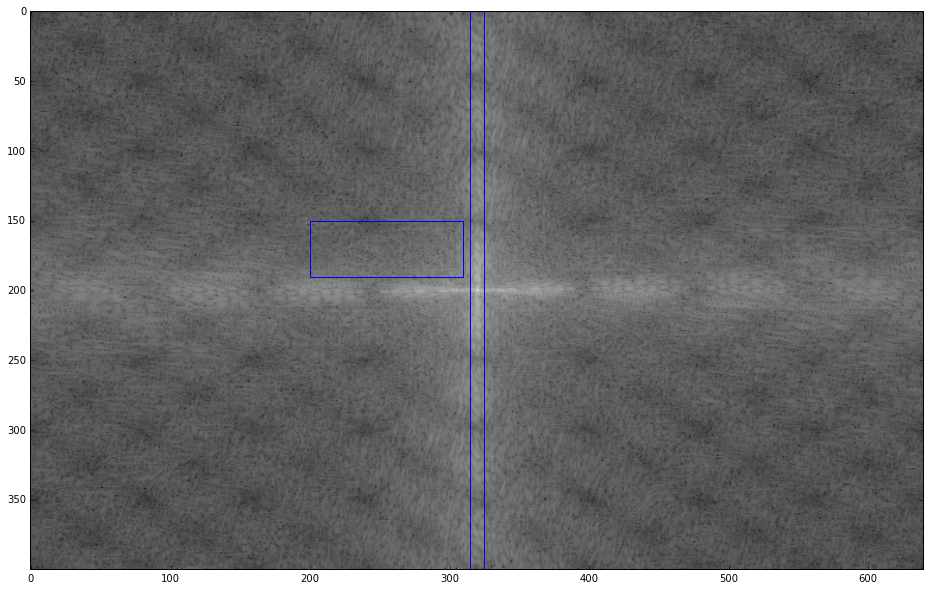
\includegraphics[scale=0.25]{fourierT}
\end{figure}

\begin{figure}[h!]
  \caption{Fourier transform of S characters}
  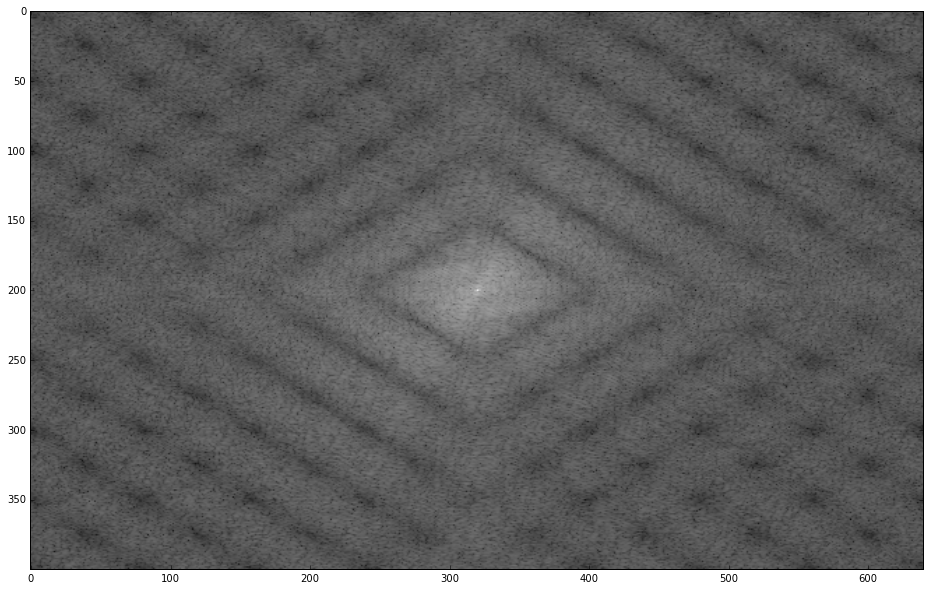
\includegraphics[scale=0.25]{fourierS}
\end{figure}

\begin{figure}[h!]
  \caption{Fourier transform of V characters}
  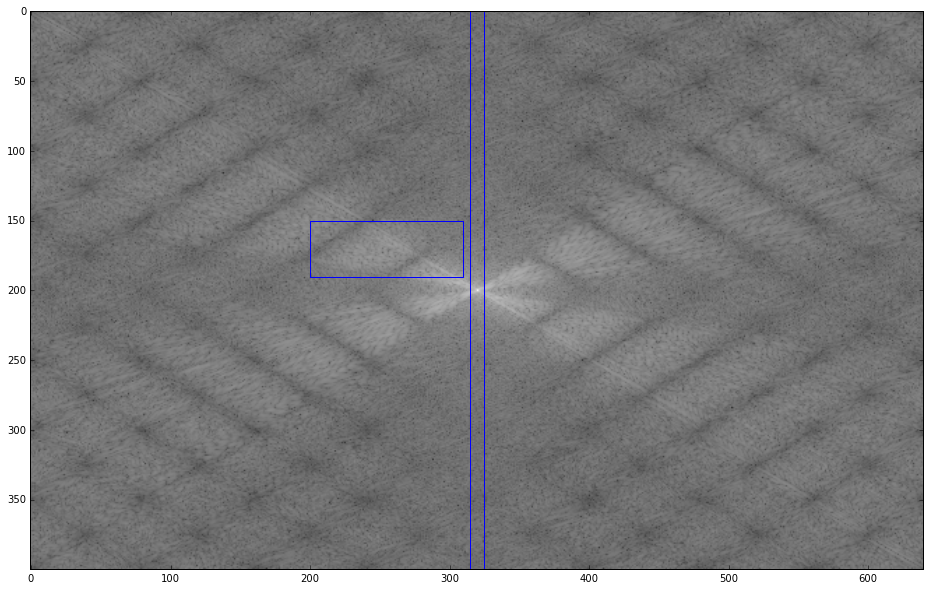
\includegraphics[scale=0.25]{fourierV}
\end{figure}




\smallskip
\newpage

Considering the three Fourier images

\justifying{
\begin{itemize}
    \item Figure 1 shows the average fourier space for the character T, from the image we
    can observe that the power spectrum has high magnitude along the vertical bar passing through the centre,
    this corresponds to the line which forms the top of character T. Similarly, there is another high magnitude bar passing horizontally
    through the centre, corresponding to the vertical part of the character

    \item Figure 2 shows the average fourier space for the character S, the power spectrum for S shows only small magnitudes for directions
    in exclusively the horizontal or vertical direction, this corresponds to the fact that a regular character S does not change in only
    the vertical or horizontal directions. As seen, the highest magnitudes lie relatively evenly distributed within the central diamond
    region, illustrative of change in both the horizontal and vertical directions, at varying angles. It is also just visible with the naked eye
    that there is a slightly more intense band in the $y=x$ line of the fourier space, this corresponds to the almost diagonal line which is part
    of some of the S test characters

    \item Figure 3 shows the average fourier space for the character V, the power spectrum shows two distinct bands in the lines $y = x$ and $y=-x$,
    the correspond to the two diagonal lines which form the letter V. We can also see the magnitude along vertical line
    passing through the centre is very low, the corresponds to the fact that there is very little change purely in the horizontal direction for the
    character V, eg the only point at which exclusively horizontal change is likely to occur is at the bottom of the character

\end{itemize}
}

\section{Choice of features}
\justifying{

    When picking features for the use of classifaction, the aim is to use regions of the
    fourier space which differ the most between fourier spaces for the given images.

    Leading on from the explanation of the fourier representation of the characters,
    the first feature I picked was a narrow vertical rectangle passing through the centre and spanning the height of the images, I reasoned that:
    The rectanlge would measure change in the horizontal direction of a image, consequently -  the overall
    magnitude spectrum within this region is largest for the letter T. Furthermore, we can observe that the amount of horizontal change
    is next largest in the S character(owing to the top and bottom near horizontal lines which are components of the S character),
    the smallest amount of horizontal change can be seen in the V character, as there is only a very small area at the bottom in which the change
    is purely horizontal.
}
    \bigskip

    The second feature chosen was a rectangular box in the top left quadrant of the image as shown, I reasoned that
    I should use a feature which did not include change in the vertical or horizontal directly exclusively.
    I reasoned that the T would have the lowest power magnitude in the region mentioned, owing to the fact that a T
    is composed of a vertical and horizontal line placed orthogonally to one another. The next highest magnitude should
    be that of the S, as seen from the Fourier space, S has a high magnitude in the central diamond region. V should have
    the highest magnitude owing to the fact it changes the most in both the horizontal and vertical directions


\section{Results of Fourier Domain analysis and analysis of the classifier}

    Using the features chosen in the previous section, I computed the sum of the power spectrum in the regions selected
    by the features for each letter. I then applied the nearest neighbour procedure with $k=1$ and uniform weighting to the list of
    values produced by the feature extraction, the results are shown in \textit{fig. 4}. The figure shows the decision regions for the
    nearest neighbour classification given a test point, the \textcolor{red}{red} region shows the area where a point will be classified as a T,
    the \textcolor{blue}{blue} region shows where a point will be classified as a S, and the \textcolor{green}{green} area shows where a point will be classified
    as a V.



    \begin{figure}[h!]
      \caption{Result of feature extraction, with decision boundaries shown}
      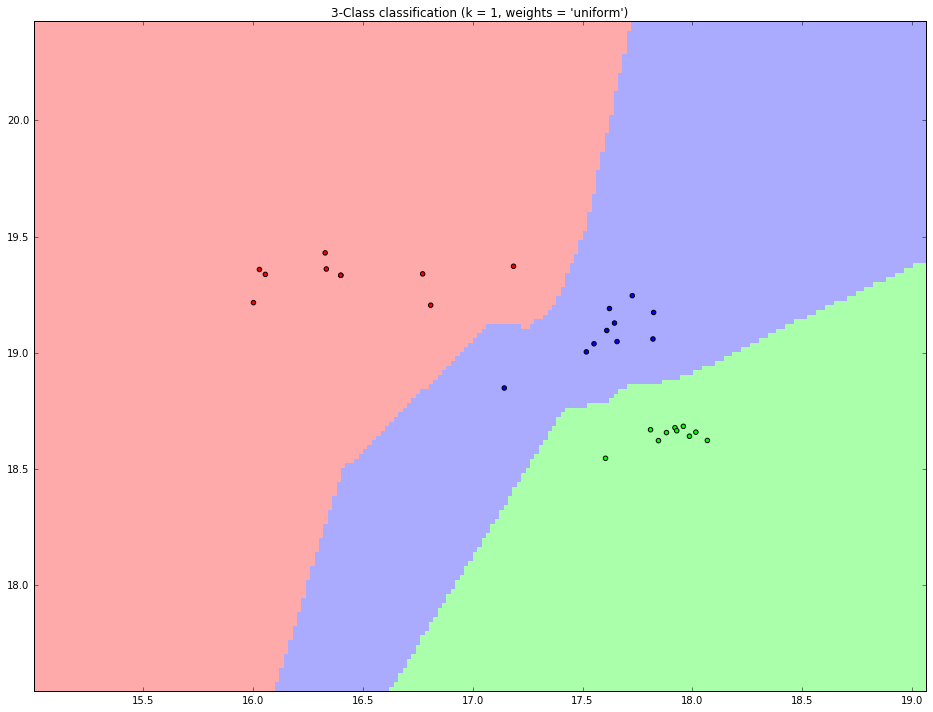
\includegraphics[scale=0.25]{decision}
    \end{figure}



    The training data produced three regions which correspond to the letters T, V and S. The clustering seems relatively good, except for
    one of the S points. Observing fig 4 we can see that one S value is far closer to the V decision boundary than the rest. I reasoned that
    the culprit would be an S which had more diagonal information in it than the others, the increased intensity in the $y = -x$ line in the fourier
    space would cause it to increasingly resemble a V. One by one I removed datapoints from the dataset and plotted the resulting nearest neighbour
    classification, I found that the culprit was \textbf{S7}.
    *picture of S7 vs superimposed images of others*

    \bigskip
    \justifying{
    To test my classifier, I created 10 new images for each character. The graph below shows the resulting classification for the points. Observing the graph
    we can see that all input Ts have been classified correctly, each T also lies relatively far way from the decision boundary between T and S. Considering
    the next character, Ss have all also been classified correctly for my test data, some of the near the decision boundary for Ss and Ts, this corresponds
    to the more horizontal tops and bottoms of some of the test Ss. my classifier classifier also correctly identified all test V characters, however
    one of test Vs was very close to the decision boundary between S and V, this is a consequence of that particular V being extremly curved.
    }
    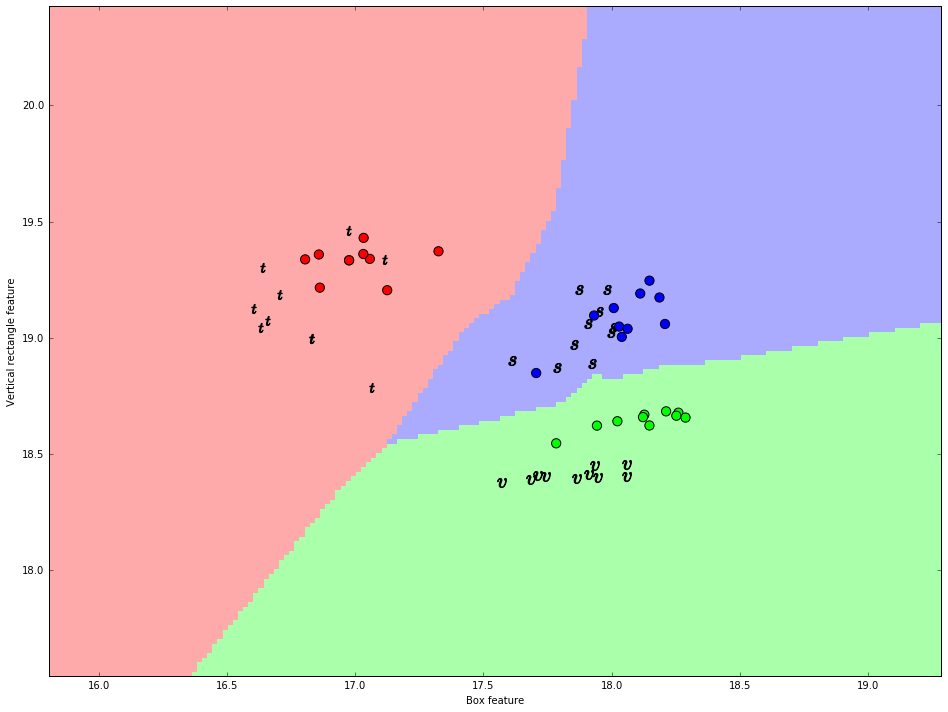
\includegraphics[scale=0.25]{testpoints}

    \bigskip
    \justifying{
    Next, I wanted to see how the classifier would cope with extreme cases for some test characters. I created the characters seen below,
    the characters seen have been drawn to any weaknesses in the chosen features
    }

        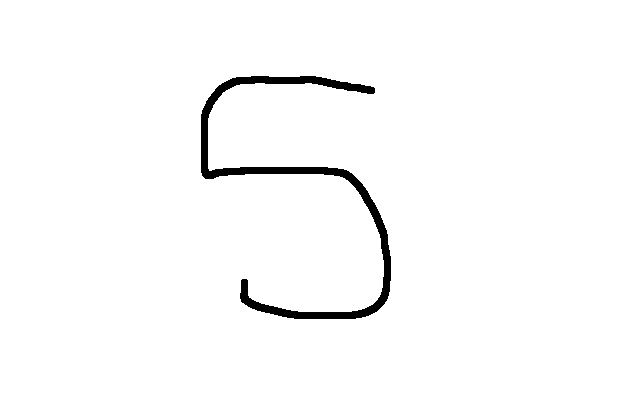
\includegraphics[scale=0.1]{tS11}
        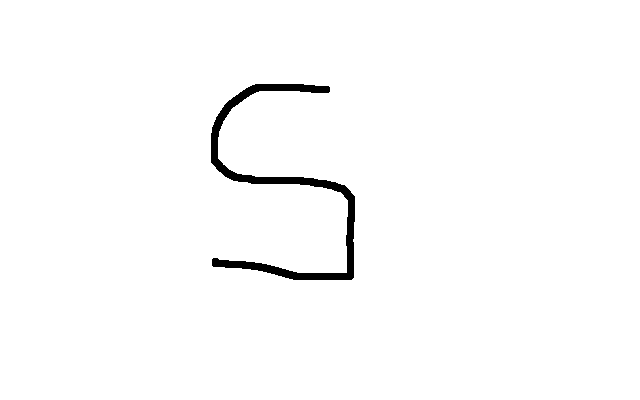
\includegraphics[scale=0.1]{tS12}
        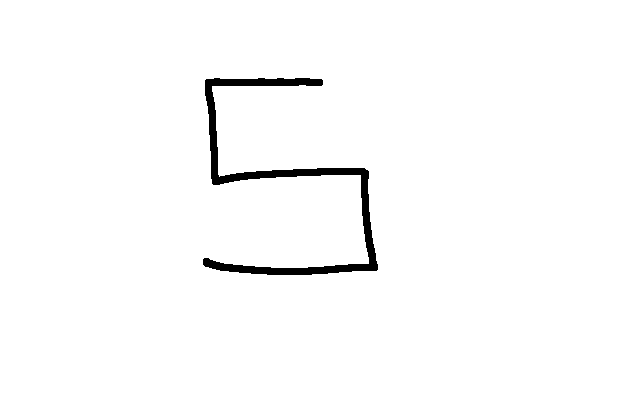
\includegraphics[scale=0.1]{tS13}
        \includegraphics[scale=0.1]{tv11}
        \includegraphics[scale=0.1]{tv12}
        \includegraphics[scale=0.1]{tv13}
        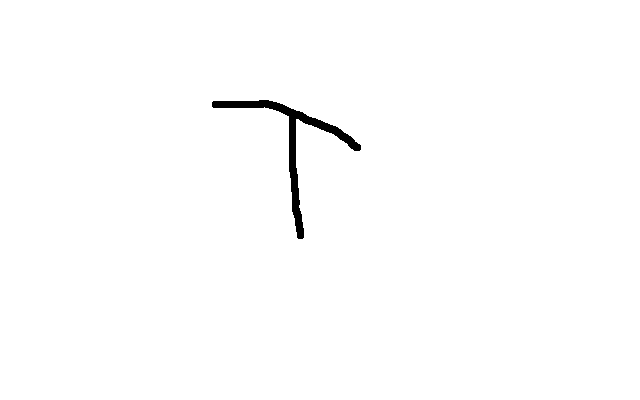
\includegraphics[scale=0.1]{tT11}
        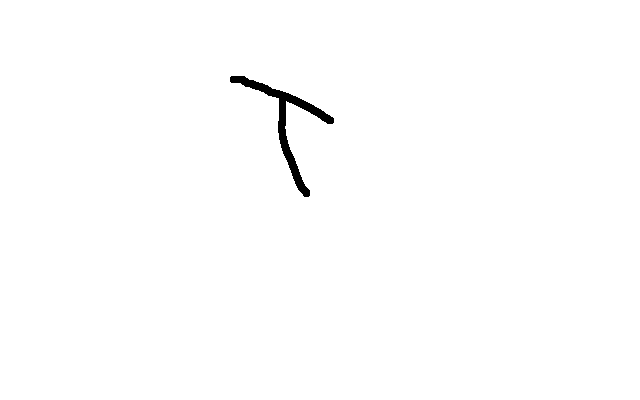
\includegraphics[scale=0.1]{tT13}
        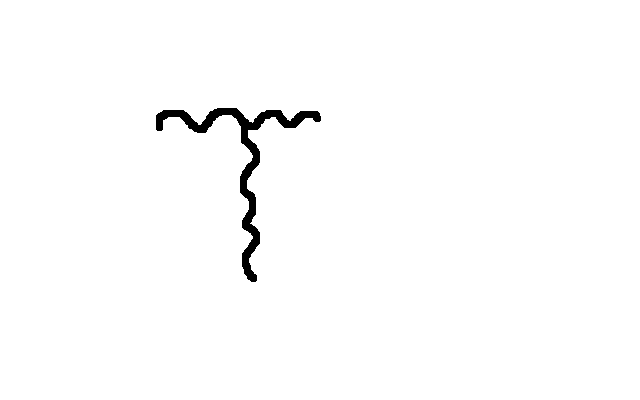
\includegraphics[scale=0.1]{tT12}

        \begin{figure}[h!]
          \caption{Assignment of extreme test characters}
          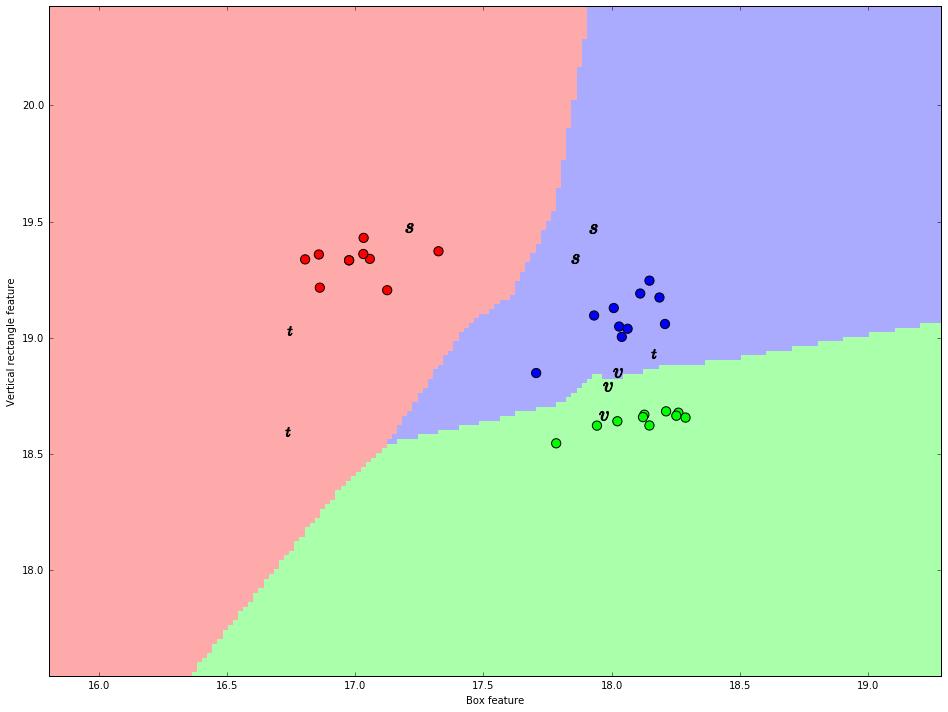
\includegraphics[scale=0.25]{extremechars}
        \end{figure}

    \justifying{

        \textit{fig 5} shows the resulting assignment of the characters seen above. Referring first to the Ss,
        observing the figure we can see that the first two Ss have been classified correctly  despite the fact that both contain
        areas of exclusive horizontal change, the small amount of curvature was enough to distinguish them from Ts. The third T, however,
        has areas almonst \textit{only} containing exclusive horizontal or vertical change, leading to its classification as a T


        \smallskip

        Considering the Ts, observing the figure we can see that two of them have been correctly classified as Ts, the points lie further
        away from the training cluster due to the fact that the Ts drawn have a much smaller horizontal component as a whole. The T composed
        of wiggly lines has been classifed as an S owing to its change magnitude in many directions.

        \smallskip
        Lastly considering the Vs, we can see from the figure that again two of them have been correctly classified, they lie very close
        to the boundary due because they contain enough horizontal change to push them in the direction of T by the first feature. This argument
        applies to why the third v is incorrectly classified as an S - the box classifier identifies it as a V, but because of the presense of
        the horizontal line, it is shifted by the first feature in the T direction, hence it is classified as an S.


    }



% \section{Analysis of the classifier}

\section{Decision region plots and their angles}

\end{flushleft}



\end{document}
